%%% use twocolumn and 10pt options with the asme2ej format
\documentclass[twocolumn,10pt]{asme2ej}
\usepackage[italian]{babel}

% \usepackage[none]{hyphenat}% don't break words

\usepackage[utf8]{inputenc}
\usepackage{epsfig} %% for loading postscript figures
\usepackage{subfigure}
\usepackage{titling}
\usepackage{multicol}
\usepackage{booktabs}
\usepackage{siunitx}
\usepackage{amsmath}
\usepackage{tikz,mathtools}
\usepackage[hidelinks]{hyperref}
\usepackage{fancyhdr}
\pagestyle{fancy}
\renewcommand{\headrulewidth}{0pt}
\fancyhead{}
\fancyfoot{}
\fancyfoot[R]{\thepage}
\usepackage{caption}
\captionsetup[table]{name=Tab.}
\captionsetup[figure]{name=Fig.}



\addto\extrasitalian{\renewcommand{\figureautorefname}{Fig.}}
\addto\extrasitalian{\renewcommand{\tableautorefname}{Tab.}}
\addto\extrasitalian{\renewcommand{\equationautorefname}{Eq.}} 
\addto\extrasitalian{\renewcommand{\sectionautorefname}{Sez.}} 
\addto\extrasitalian{\renewcommand{\subsectionautorefname}{Sez.}}
\addto\extrasitalian{\renewcommand{\subsubsectionautorefname}{Sez.}}


\pretitle{\begin{center}\linespread{1.2}\huge}
\posttitle{\par\end{center}\vspace{0.5em}}

\abovedisplayshortskip=0pt
\belowdisplayshortskip=0pt
\abovedisplayskip=-5pt
\belowdisplayskip=5pt

\newcommand{\tnhl}{\tabularnewline\hline}
\newcommand{\tn}{\tabularnewline}
\newcolumntype{C}[1]{%
	>{\centering\hspace{0pt}}p{#1}}%
\newcolumntype{L}[1]{%
	>{\raggedright\hspace{0pt}}p{#1}}%
\newcolumntype{R}[1]{%
	>{\raggedleft\hspace{0pt}}p{#1}}%



%% The class has several options
%  onecolumn/twocolumn - format for one or two columns per page
%  10pt/11pt/12pt - use 10, 11, or 12 point font
%  oneside/twoside - format for oneside/twosided printing
%  final/draft - format for final/draft copy
%  cleanfoot - take out copyright info in footer leave page number
%  cleanhead - take out the conference banner on the title page
%  titlepage/notitlepage - put in titlepage or leave out titlepage
%  
%% The default is oneside, onecolumn, 10pt, final

\date{}
\title{{\huge\bfseries Laboratorio di Fisica} - {\LARGE A.A. 2020/2021} \\ 
    {\LARGE Docenti: A. Garfagnini - M. Lunardon} \\ {\Huge\bfseries Fotodiodo}}


%%% first author
\author{Cerrone Vanessa
    \affiliation{
    1200361\\
    vanessa.cerrone@studenti.unipd.it
    }	
}

%%% second author
\author{Cigagna Simone
    \affiliation{
	1193992\\
    simone.cigagna@studenti.unipd.it
    }	
}

%%% third author
\author{Lai Nicolò
    \affiliation{
	1193976\\
    nicolo.lai@studenti.unipd.it
    }	
}


\begin{document}


\maketitle    


% %%%%%%%%%%%%%%%%%%%%%%%%%%%%%%%%%%%%%%%%%%%%%%%%%%%%%%%%%%%%%%%%%%%%%%
\section{Introduzione}\label{s:introduzione}

L'esperienza consiste nell'analisi dello spettro dei fotoni emessi dall'Americio-241 con un rivelatore al Silicio tipo
PIN, dotato di preamplificatore di carica. L'hardware, cioè i moduli di elettronica, sono stati pre-impostati in
condizioni standard, con shaping time pari a $3\,\si{\micro\second}$, in modo da ottimizzare il rapporto segnale rumore.

Inizialmente, in \autoref{s:spettro}, si propone un'analisi dettagliata dello spettro di emissione dell'Am-241: in
particolare, dopo una calibrazione approssimativa in energia, si fornisce una stima per la risoluzione energetica per la
rivelazione di raggi $\gamma$ e un tentativo di fit dell'intero profilo dello spettro. Successivamente, in
\autoref{s:attenuazione}, si interpongono tra la sorgente ed il rivelatore degli assorbitori di materiale e spessore
differenti al fine di verificare gli effetti dell'interazione radiazione-materia, confrontando i coefficienti di
assorbimento stimabili dall'analisi degli spettri con i valori teorici. In \autoref{s:distanza}, invece, si è
intenzionati a verificare la legge dell'inverso del quadrato della distanza, acquisendo lo spettro di emissione al
variare della posizione del detector. Infine, in \autoref{s:efficienza}, si studia l'efficienza relativa del detector al
variare della distanza tra quest'ultimo e la sorgente, dello spessore degli assorbitori e dell'energia dei fotoni
rivelati.


\vspace{-20pt}
% %%%%%%%%%%%%%%%%%%%%%%%%%%%%%%%%%%%%%%%%%%%%%%%%%%%%%%%%%%%%%%%%%%%%%%
\section{Spettro dell'Am-241}\label{s:spettro}

Prima di studiare in dettaglio gli effetti di diversi assorbitori posti tra la sorgente ed il detector ed il ruolo che
svolge la distanza di quest'ultimo dalla prima, ci si vuole concentrare sull'analisi dello spettro dell'Americio-241.
Sperimentalmente, il rivelatore viene posto alla minima distanza dalla sorgente e non viene inserito alcun assorbitore
tra i due. Il tempo di acquisizione viene impostato a $600\,\si{\second}$, rivelando così approssimativamente $2 \cdot
10^5$ eventi con un rate istantaneo di circa $340\,\si{\hertz}$. In questo modo, il picco a
$60\,\si{\kilo\electronvolt}$ presenta una precisione $\sqrt{\text{N}}/\text{N} \approx 1.5\%$.

\subsection{Calibrazione e Risoluzione Energetica}\label{s:calibrazione}

Inizialmente, si vuole calibrare l'asse orizzontale riconoscendo nello spettro in \autoref{i:spettro} il picco a
$60\,\si{\kilo\electronvolt}$. Nel grafico è presentato lo spettro di emissione con l'asse calibrato in energia: per
ottenere tale risultato è stato eseguito un fit gaussiano del picco, come mostrato nel riquadro all'interno del grafico.
Ovviamente, la calibrazione ottenuta sfruttando unicamente il picco a $60\,\si{\kilo\electronvolt}$ e assumendo
l'assenza di un possibile offset è approssimata, tuttavia risulta essere sufficiente per gli scopi dell'esperienza. 

\begin{figure}
    \centering
    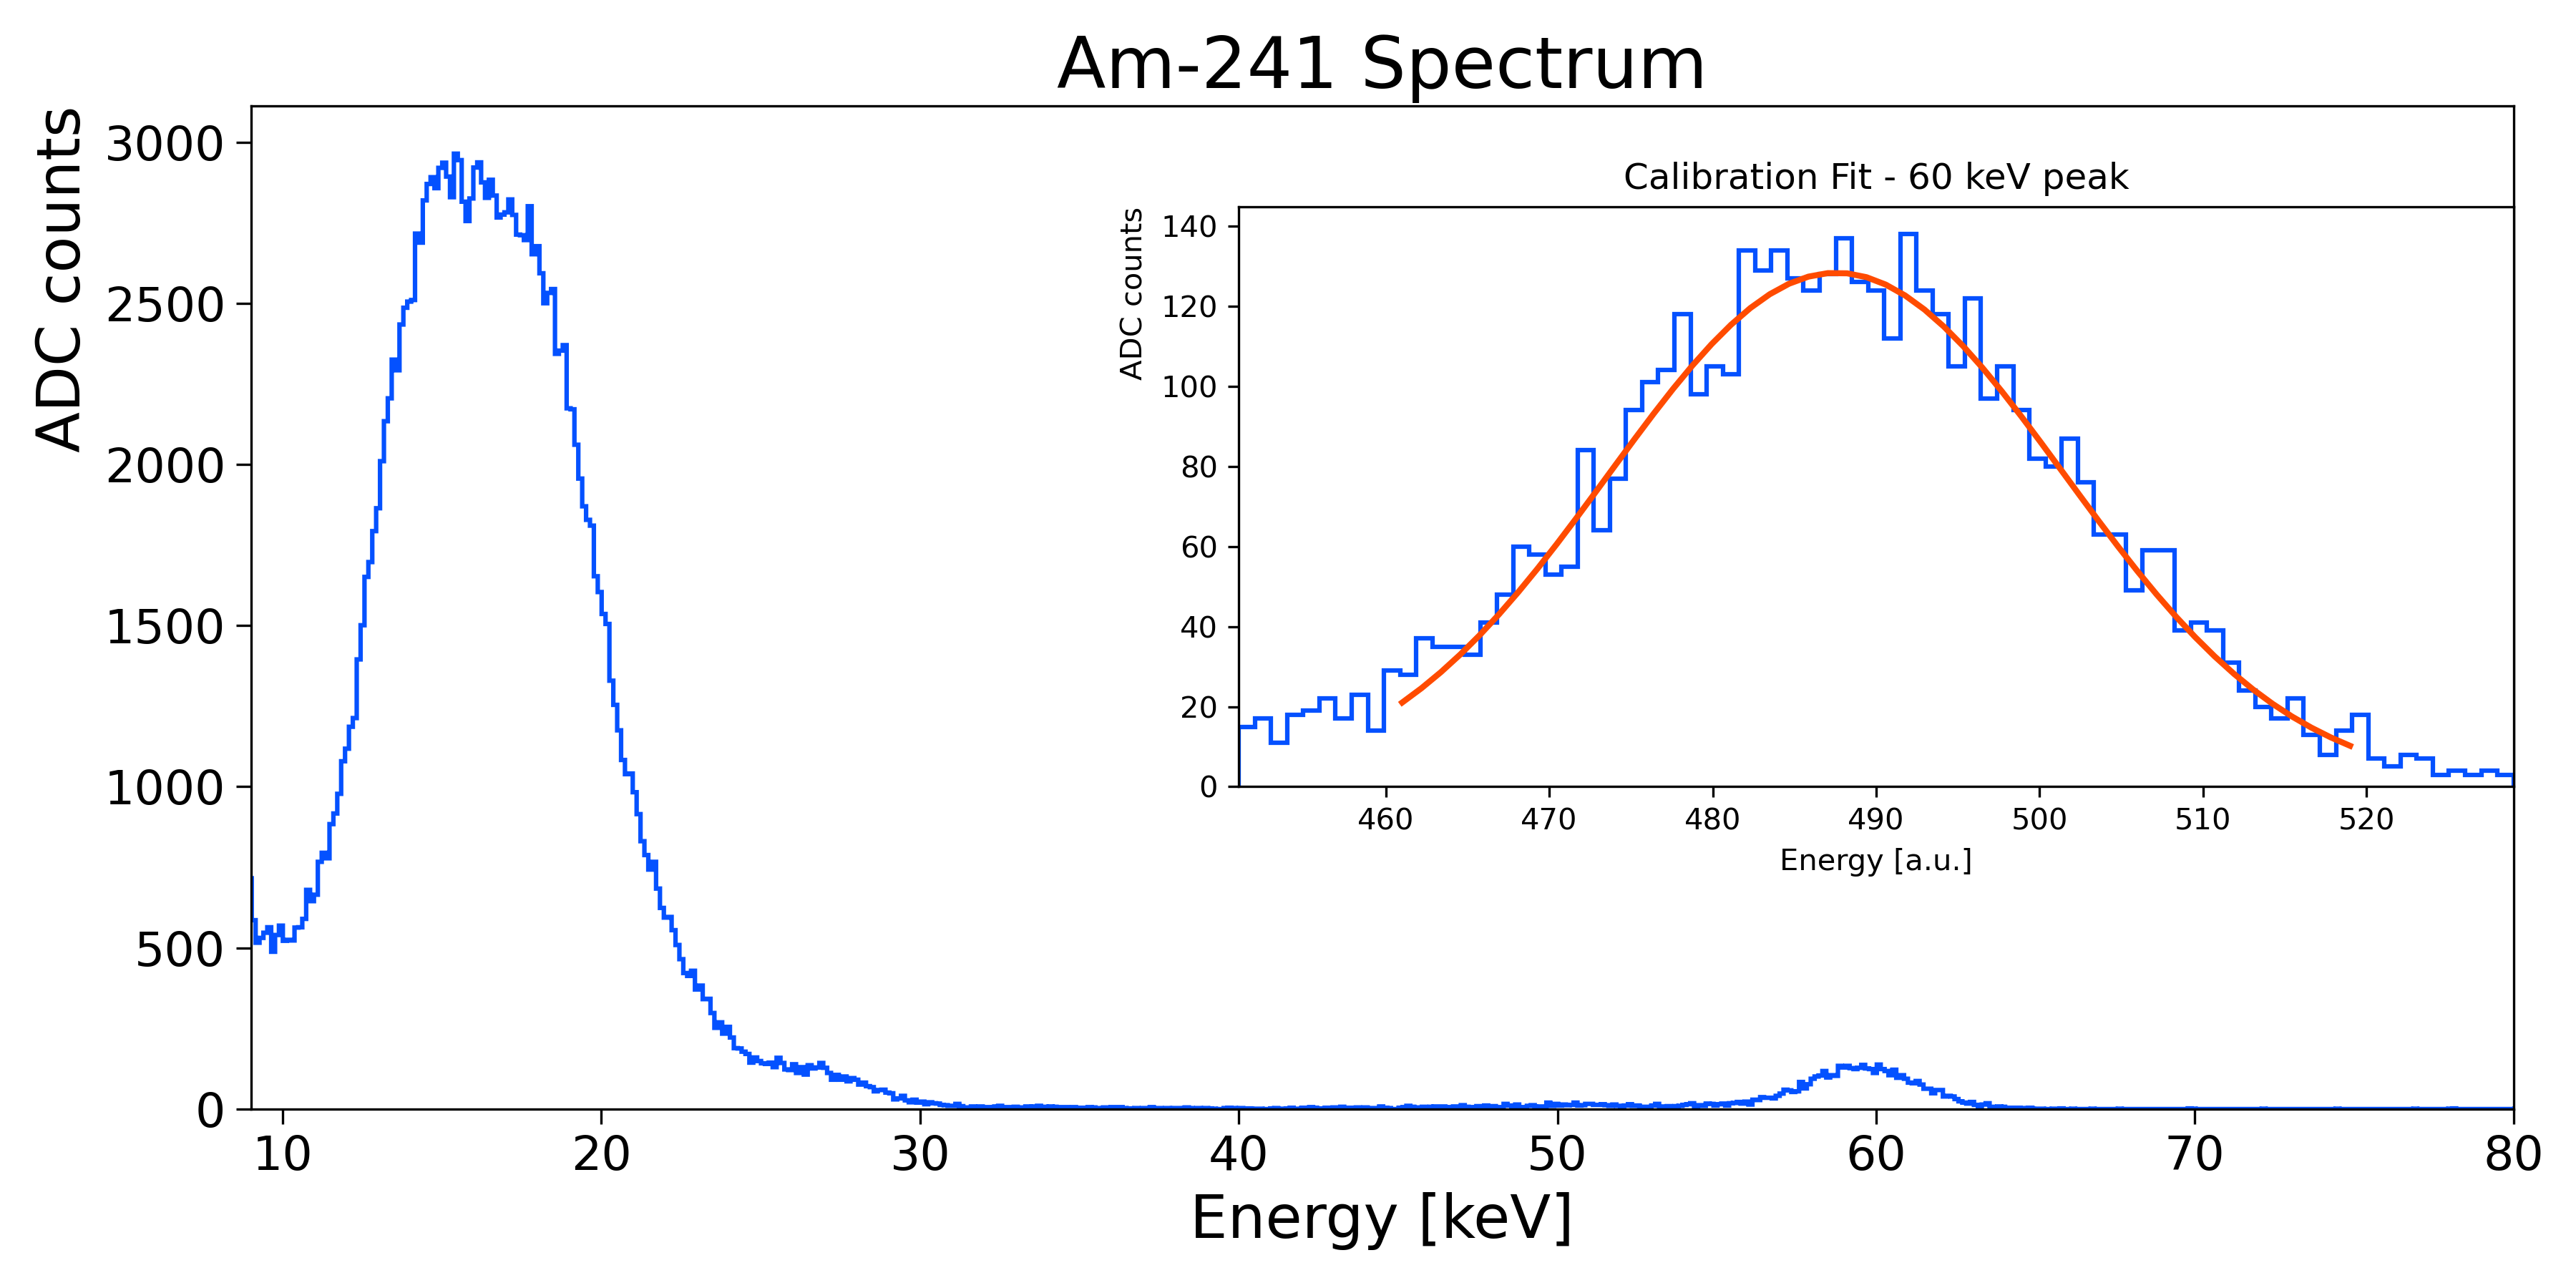
\includegraphics[width=\linewidth]{../Plots/am_spectrum_small.png}
    \caption{Spettro dell'Americio-241 con fit del picco a 60 keV per la calibrazione
               dell'asse orizzontale}
    \label{i:spettro}
    \vspace{-10pt}
\end{figure}

Dal fit del picco a $60\,\si{\kilo\electronvolt}$ è possibile infine estrapolare una stima approssimata della
risoluzione energetica R: 

\vspace{-15pt}
\begin{equation}
    \text{R} = \frac{\Delta\text{E}}{\text{E}}
    \underset{\mathllap{
      \begin{tikzpicture}
        \draw[->] (-0.3, 0) to[bend right=20] ++(0.3,2ex);
        \node[below left] at (0,0) {in assenza di offset};
      \end{tikzpicture}
    }}{\simeq}
    \frac{\text{FWHM}}{\text{mean}} = 6.75\%
\vspace{-5pt}
\end{equation}


\subsection{Fit Multi-Picco}\label{s:multipicco}

\begin{figure*}
    \centering
    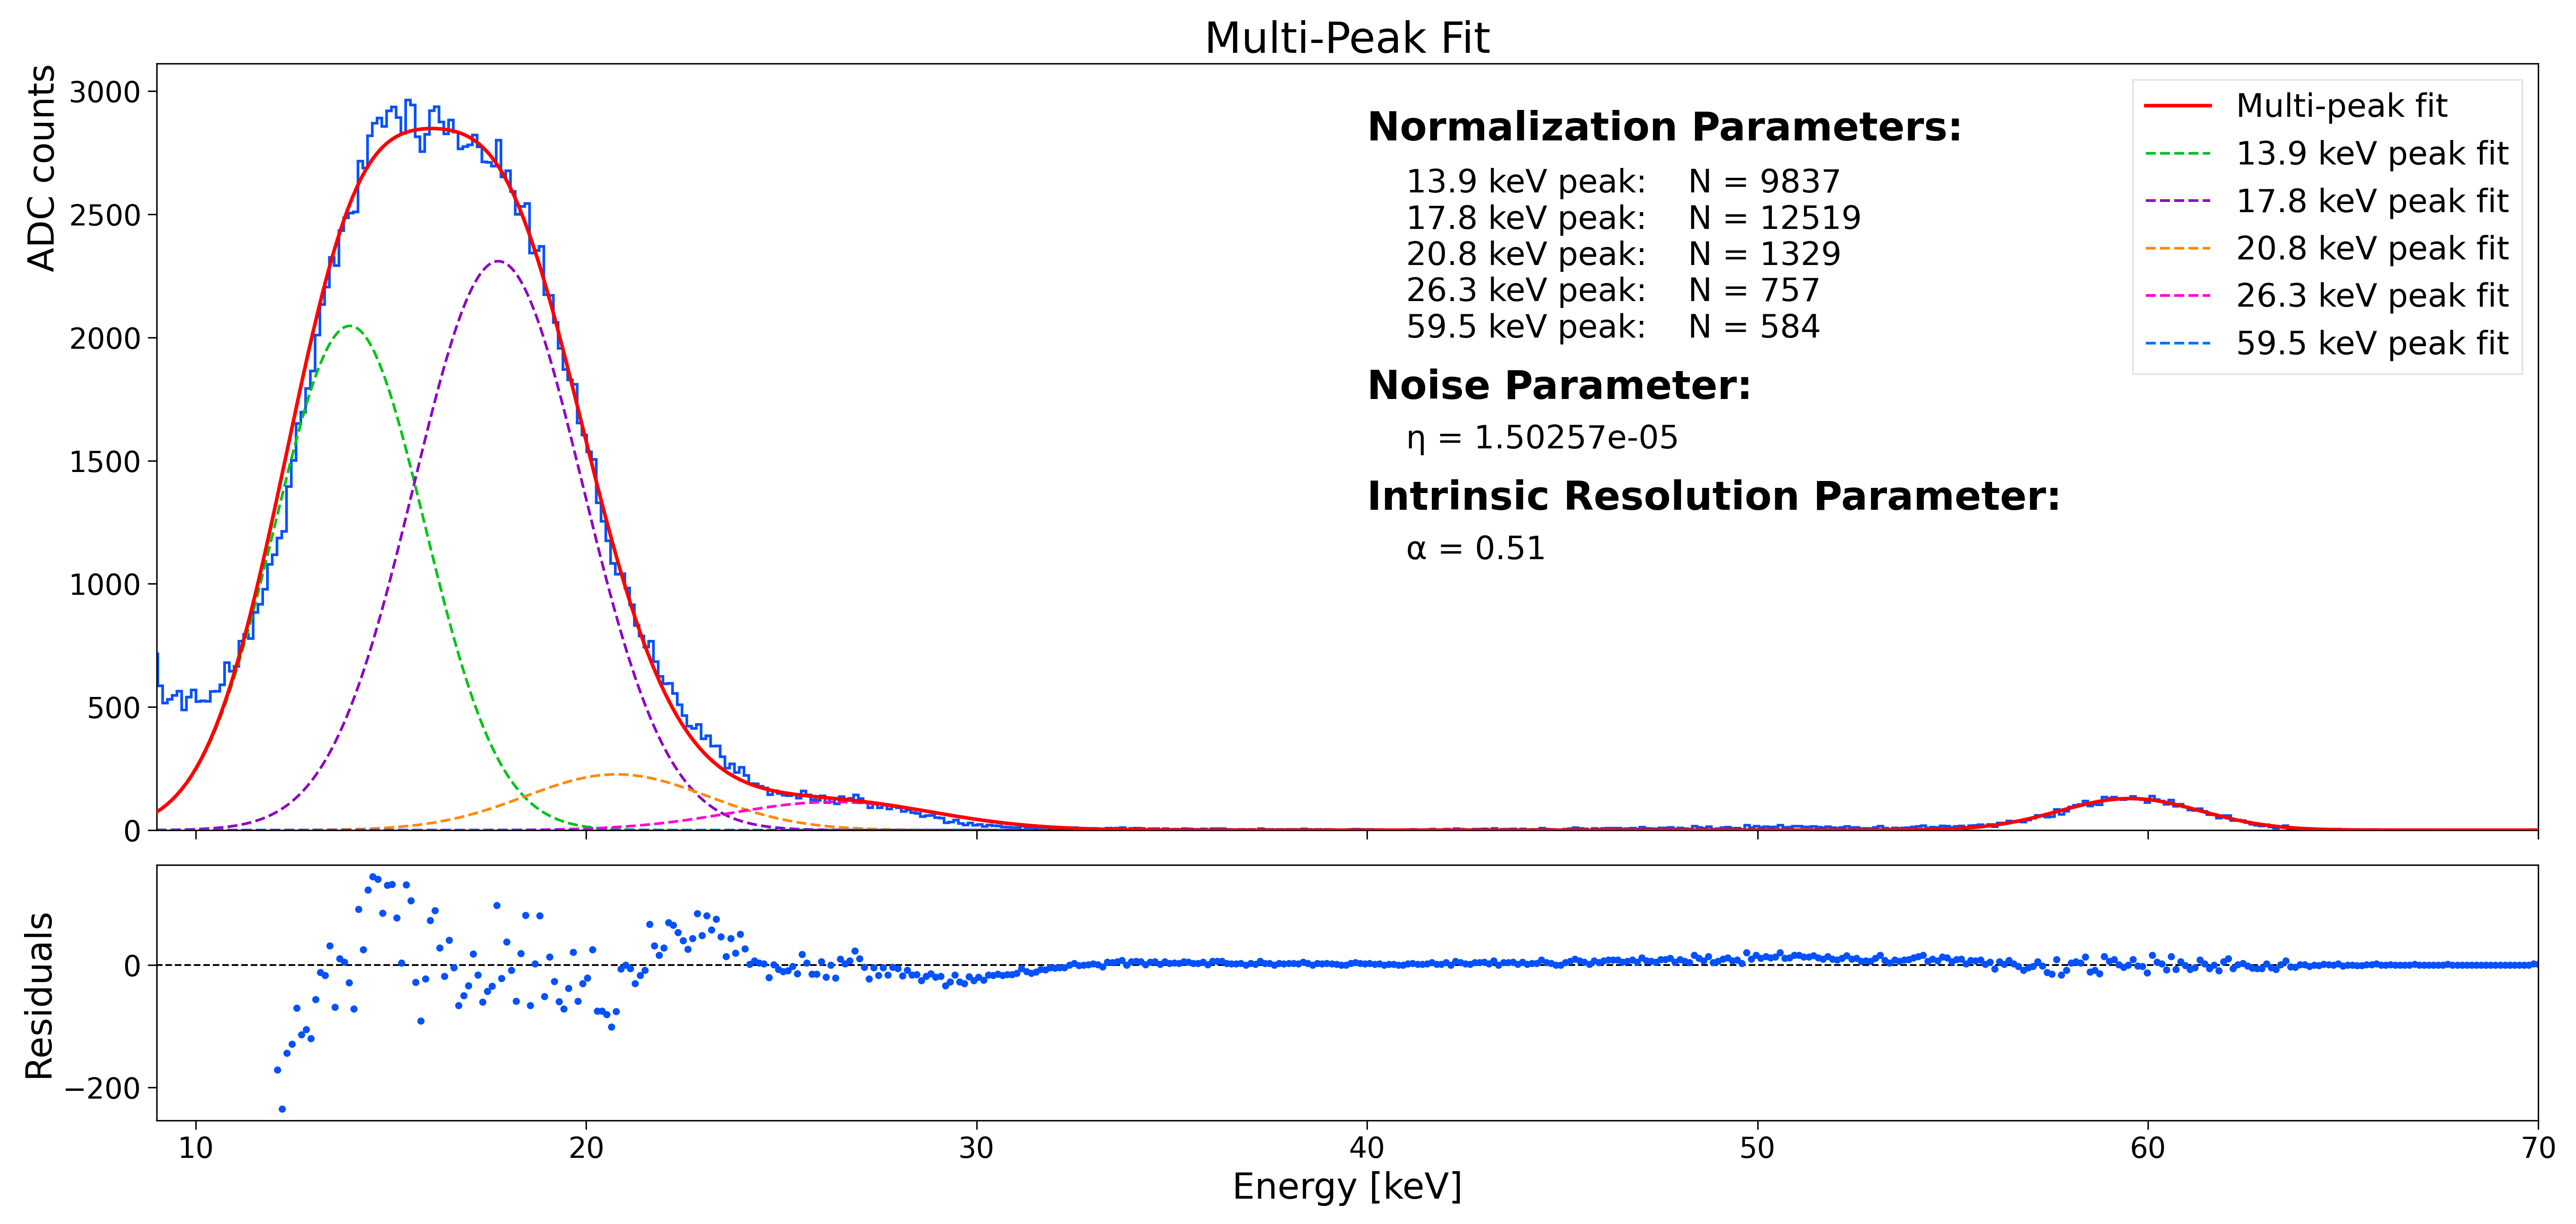
\includegraphics[width=\textwidth]{../Plots/multifit.png}
   \caption{Fit multi-picco dello spettro dell'Americio-241}
    \label{i:multifit}
    % \vspace{-10pt}
\end{figure*}

Ci si propone ora di costruire un fit complessivo di tutto lo spettro raffigurato in \autoref{i:spettro}. Ci si
concentra unicamente sulle emissioni di raggi X e gamma con un'intensità di almeno 2 fotoni ogni 100 disintegrazioni: in
\autoref{t:probabilities} sono riportati quindi i contributi considerati con le relative probabilità di emissione. Per
ciascuno di questi, si costruisce una funzione gaussiana con media fissata, in quanto l'energia è nota
(\autoref{t:probabilities}), con l'asse orizzontale preliminarmente calibrato. La larghezza della gaussiana (sigma),
invece, si compone di due contributi in somma quadratica: il primo è una componente fissa, di rumore, che verrà denotata
come $\eta$, mentre il secondo è la componente di risoluzione intrinseca, proporzionale alla radice quadrata
dell'energia del fotone preso in considerazione. La funzione fittante è quindi data dalla somma delle sei gaussiane,
ottendendo in questo modo quanto raffigurato in \autoref{i:multifit}. In particolare, sono stati scelti come parametri
liberi il contributo di rumore $\eta$ e la costante di proporzionalità $\alpha$ della risoluzione intrinsceca, assieme
ai fattori di normalizzazione $\{\text{N}_i\}$ relativi ad ogni singolo picco considerato. Osservando quindi il grafico
in \autoref{i:multifit}, la curva in rosso rappresenta il fit complessivo dello spettro: questa segue in modo più che
soddisfacente il profilo delle emissioni dell'Am-241. Le curve tratteggiate, invece, corrispondono ai singoli contributi
gaussiani considerati per effettuare il fit: risulta quindi evidente che il potere risolutivo dell'apparato non è
sufficiente per identificare tali contributi singolarmente. Dal grafico dei residui, relativi al fit complessivo, si può
notare una certa difficoltà nel seguire in modo fedele il profilo del primo picco, in quanto composto da numerosi
contributi. Il picco a $60\,\si{\kilo\electronvolt}$, invece, risulta in maggiore accordo con la funzione di
regressione. I coefficienti di normalizzazione dei singoli contributi gaussiani restituiti dal fit seguono piuttosto
fedelmente l'andamento della probabilità di emissione di un fotone con tale energia, ad eccezione dei due picchi a
$16.8\,\si{\kilo\electronvolt}$ e $20.8\,\si{\kilo\electronvolt}$ che risultano essere leggermente più alti delle
aspettative: conseguentemente il contributo a $17.8\,\si{\kilo\electronvolt}$ viene sottostimato. Questa anomalia non
sorprende in quanto, a causa del basso potere risolvente dell'apparato, il fit di sei contributi gaussiani sotto un
unico picco risulta essere decisamente complicato. Il parametro di rumore $\eta$, infine, risulta essere trascurabile
rispetto al fattore di risoluzione intrinseca che si può considerare quindi il contributo predominante della sigma. 


\begin{table}[t]
	\centering
	\begin{tabular}{C{3cm} C{3cm}} 

        \toprule[0.5px]
        \toprule[0.1px]

		\multicolumn{2}{c}{\bfseries Probabilità di Emissione} \tn

		\midrule[0.1px]

		Energia [keV] & Prob. (\%) \tn

		\addlinespace

		13.9    & 11.60 (12)    \tn
        16.8    & 2.45 (26)    \tn
        17.8    & 11.83 (12)    \tn
        20.8    & 2.94 (3)      \tn
        26.3    & 2.31 (8)      \tn
        59.5    & 35.92 (17)    \tn

		\bottomrule[0.5px]		
	\end{tabular}
	\caption{Energie dei fotoni considerati nel fit multi-picco e relative probabilità di emissione}
	\label{t:probabilities}
    \vspace{-10pt}
\end{table}	




\vspace{-10pt}
% %%%%%%%%%%%%%%%%%%%%%%%%%%%%%%%%%%%%%%%%%%%%%%%%%%%%%%%%%%%%%%%%%%%%%%
\section{Coefficiente di assorbimento}\label{s:attenuazione} 

\begin{figure*}[t]
    \centering
    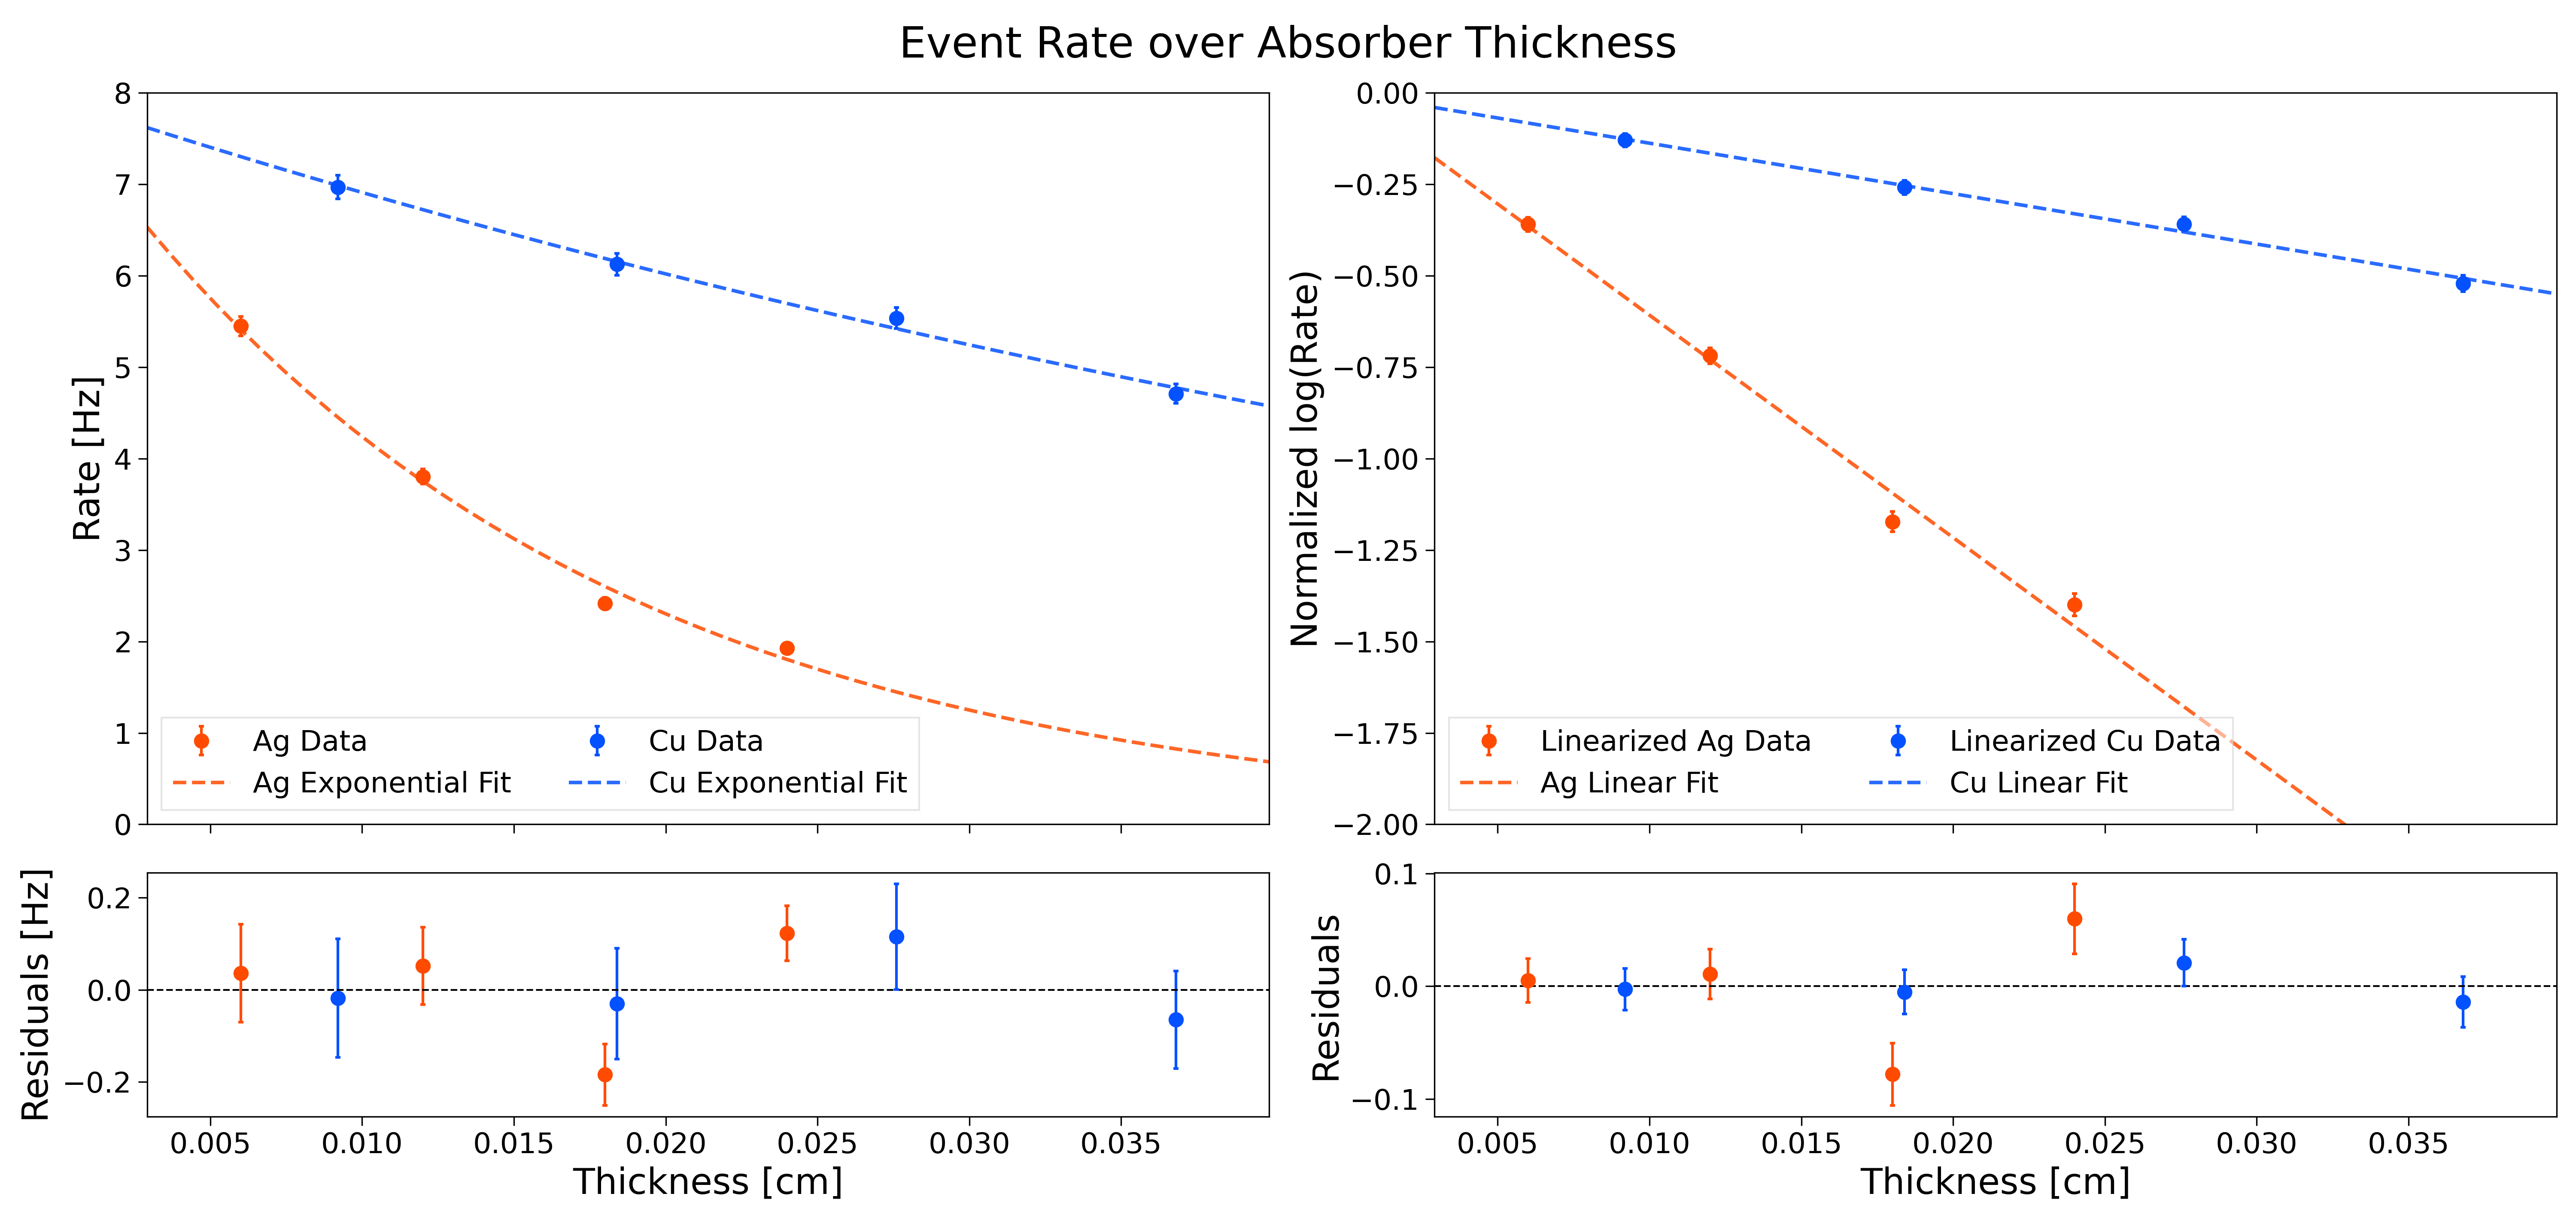
\includegraphics[width=\textwidth]{../Plots/attenuation_coeff.png}
   \caption{A sinistra fit esponenziale, a destra fit linearizzato per il calcolo dei coefficienti di assorbimento}
    \label{i:attenuation}
    % \vspace{-10pt}
\end{figure*}

\begin{table*}[t]

    \centering
    \begin{tabular}{C{1.3cm}C{1.5cm}C{1.1cm}C{1.3cm}C{1.5cm}C{1.1cm}|C{1.5cm}C{1.1cm}C{1.5cm}C{1.1cm}}

    \toprule[0.5px] 
    \toprule[0.1px]

    \multicolumn{6}{c}{Fit esponenziale} & \multicolumn{4}{c}{Fit lineare}       \tn

    \multicolumn{3}{c}{\textbf{Ag}} & \multicolumn{3}{c}{\textbf{Cu}} & 
    \multicolumn{2}{c}{\textbf{Ag}} & \multicolumn{2}{c}{\textbf{Cu}} \tn 

    \midrule[0.1px]

    $\text{I}_0$ [$\si{\hertz}$] & $\mu$ [$\si{\centi\metre^{-1}}$] & $\chi^2 / \text{ndf}$ & 
    $\text{I}_0$ [$\si{\hertz}$]& $\mu$ [$\si{\centi\metre^{-1}}$] & $\chi^2 / \text{ndf}$ & 
    $\mu$ [$\si{\centi\metre^{-1}}$] & $\chi^2 / \text{ndf}$ & 
    $\mu$ [$\si{\centi\metre^{-1}}$]  & $\chi^2 / \text{ndf}$ \tn
    
    \addlinespace

    $7.8 \pm 0.2$ & $61.1 \pm 1.9$ & $12.3 / 2$ & $7.9 \pm 0.2$ & $13.8 \pm 1.0$ & $1.5 / 2$ & $60.8 \pm 0.8$ & $12.0 /3 $ &
    $13.8 \pm 0.4$ & $1.5 / 3 $\tn 
    
    \bottomrule[0.5px]

    \end{tabular}
    \caption{Parametri fit esponenziale e lineare per il calcolo del coefficiente di assorbimento}
    \label{t:parametri_mu}
    \vspace{-10pt}
\end{table*}

Interessati all'interazione radiazione-materia, si acquisiscono gli spettri di emissione dell'Am-241 in presenza di
assorbitori di rame o argento interposti tra sorgente e detector, avendo cura di utilizzare un tempo di raccolta
sufficiente da garantire una precisione migliore del $3\%$ sul picco a $60\,\si{\kilo\electronvolt}$. Dall'analisi di
tali acquisizioni si vogliono calcolare i coefficienti di assorbimento $\mu$ propri dei due materiali: sussiste infatti
la relazione

\vspace{-15pt}
\begin{equation}
   \text{I}(x) = \text{I}_0 \text{e}^{-\mu x}
    \label{e:mu}
    \vspace{-5pt}
\end{equation}

\noindent dove I è l'intensità della radiazione rivelata dal detector, $\text{I}_0$ corrisponde all'intensità della
radiazione incidente sull'assorbitore mentre $x$ è lo spessore attraversato (in seguito denotato come $d$). In
particolare, si vuole fornire una stima del coefficiente di assorbimento massivo, definito come:

\vspace{-15pt}
\begin{equation}
   \mu_{\rho} = \frac{\mu}{\rho}
    \vspace{-5pt}
    \label{e:mu_mass}
\end{equation}

\noindent dove $\rho$ rappresenta la densità del materiale. 

Sapendo che il numero di fotoni per unità di tempo (rate) e superficie è pari al rapporto tra l'intensità della
radiazione e l'energia del fotone, sussiste una relazione analoga ad \autoref{e:mu} per il rate, facilmente calcolabile
dall'acquisizione degli spettri di emissione. Di conseguenza, il rate di rivelazione dei raggi $\gamma$ a
$60\,\si{\kilo\electronvolt}$ viene computato come rapporto tra numero di eventi rivelati in un range fissato per tutti
gli spettri e tempo di acquisizione. Per la stima del coefficiente di assorbimento $\mu$, si decide di predisporre un
fit delle misure di rate al variare dello spessore $d$ dell'assorbitore. È opportuno sottolineare che, a seconda del
materiale, vengono considerati due dataset distinti. 

\begin{table}[t]
    \begin{center}
        \begin{tabular}{C{1.5cm} C{1.8cm} | C{1.5cm} C{1.8cm}}
            \toprule[0.5px]
            \toprule[0.1px]
            \multicolumn{2}{c}{\textbf{Ag}} & \multicolumn{2}{c}{\textbf{Cu}} \tn
            \midrule[0.1px]
            d [$\si{\micro\metre}$] & Rate [Hz] & d [$\si{\micro\metre}$] & Rate [Hz] \tn
            \addlinespace
            60      & $5.45  \pm  0.11$    & 92       & $6.97 \pm 0.13$   \tn
            120     & $3.80  \pm  0.08$    & 184      & $6.12 \pm 0.12$   \tn
            180     & $2.42  \pm  0.07$    & 276      & $5.54 \pm 0.11$   \tn
            240     & $1.93  \pm  0.06$    & 368      & $4.71 \pm 0.11$   \tn  
            \bottomrule[0.5px]	
        \end{tabular}
    \end{center}
    \caption{Spessore dell'assorbitore e relativo rate di rivelazione divisi per materiale}
    \label{t:assorbimento}
    \vspace{-10pt}
\end{table}

\begin{table*}[t]
	\centering
	\begin{tabular}{L{6.5cm} C{4.7cm} C{4.7cm}} 

        \toprule[0.5px]
        \toprule[0.1px]

		\multicolumn{3}{c}{\bfseries Coefficienti di assorbimento} \tn

		\midrule[0.1px]

		& Argento & Rame\tn

        \addlinespace

        Coefficiente di assorbimento            &  
        $\mu = 60.8 \pm 0.8   \,\si{\centi\metre^{-1}}$ &
        $\mu = 13.8 \pm 0.4  \,\si{\centi\metre^{-1}}$
        \tn
        Densità del materiale                   &  
        $\rho = 10.49  \,\si{\gram\centi\metre^{-3}}$  & 
        $\rho = 8.96  \,\si{\gram\centi\metre^{-3}}$  \tn
        Coefficiente di assorbimento massivo    &  
        $\mu_{\rho} = 5.82 \pm 0.18 \,\si{\centi\metre^2\gram^{-1}}$ & 
        $\mu_{\rho} = 1.54 \pm 0.11 \,\si{\centi\metre^2\gram^{-1}}$ \tn
        Aspettativa teorica                     &  
        $\mu_{\rho}^{\text{th}} = 5.766  \,\si{\centi\metre^2\gram^{-1}}$ & 
        $\mu_{\rho}^{\text{th}} = 1.593  \,\si{\centi\metre^2\gram^{-1}}$  \tn
        Compatibilità                           & 
        $\lambda = 0.3$ &
        $\lambda = 0.5$    \tn 

		\bottomrule[0.5px]		
	\end{tabular}
	\caption{Coefficienti di assorbimento: valori teorici e stime sperimentali}
	\label{t:results}
    \vspace{-10pt}
\end{table*}

\begin{figure}
    \centering
    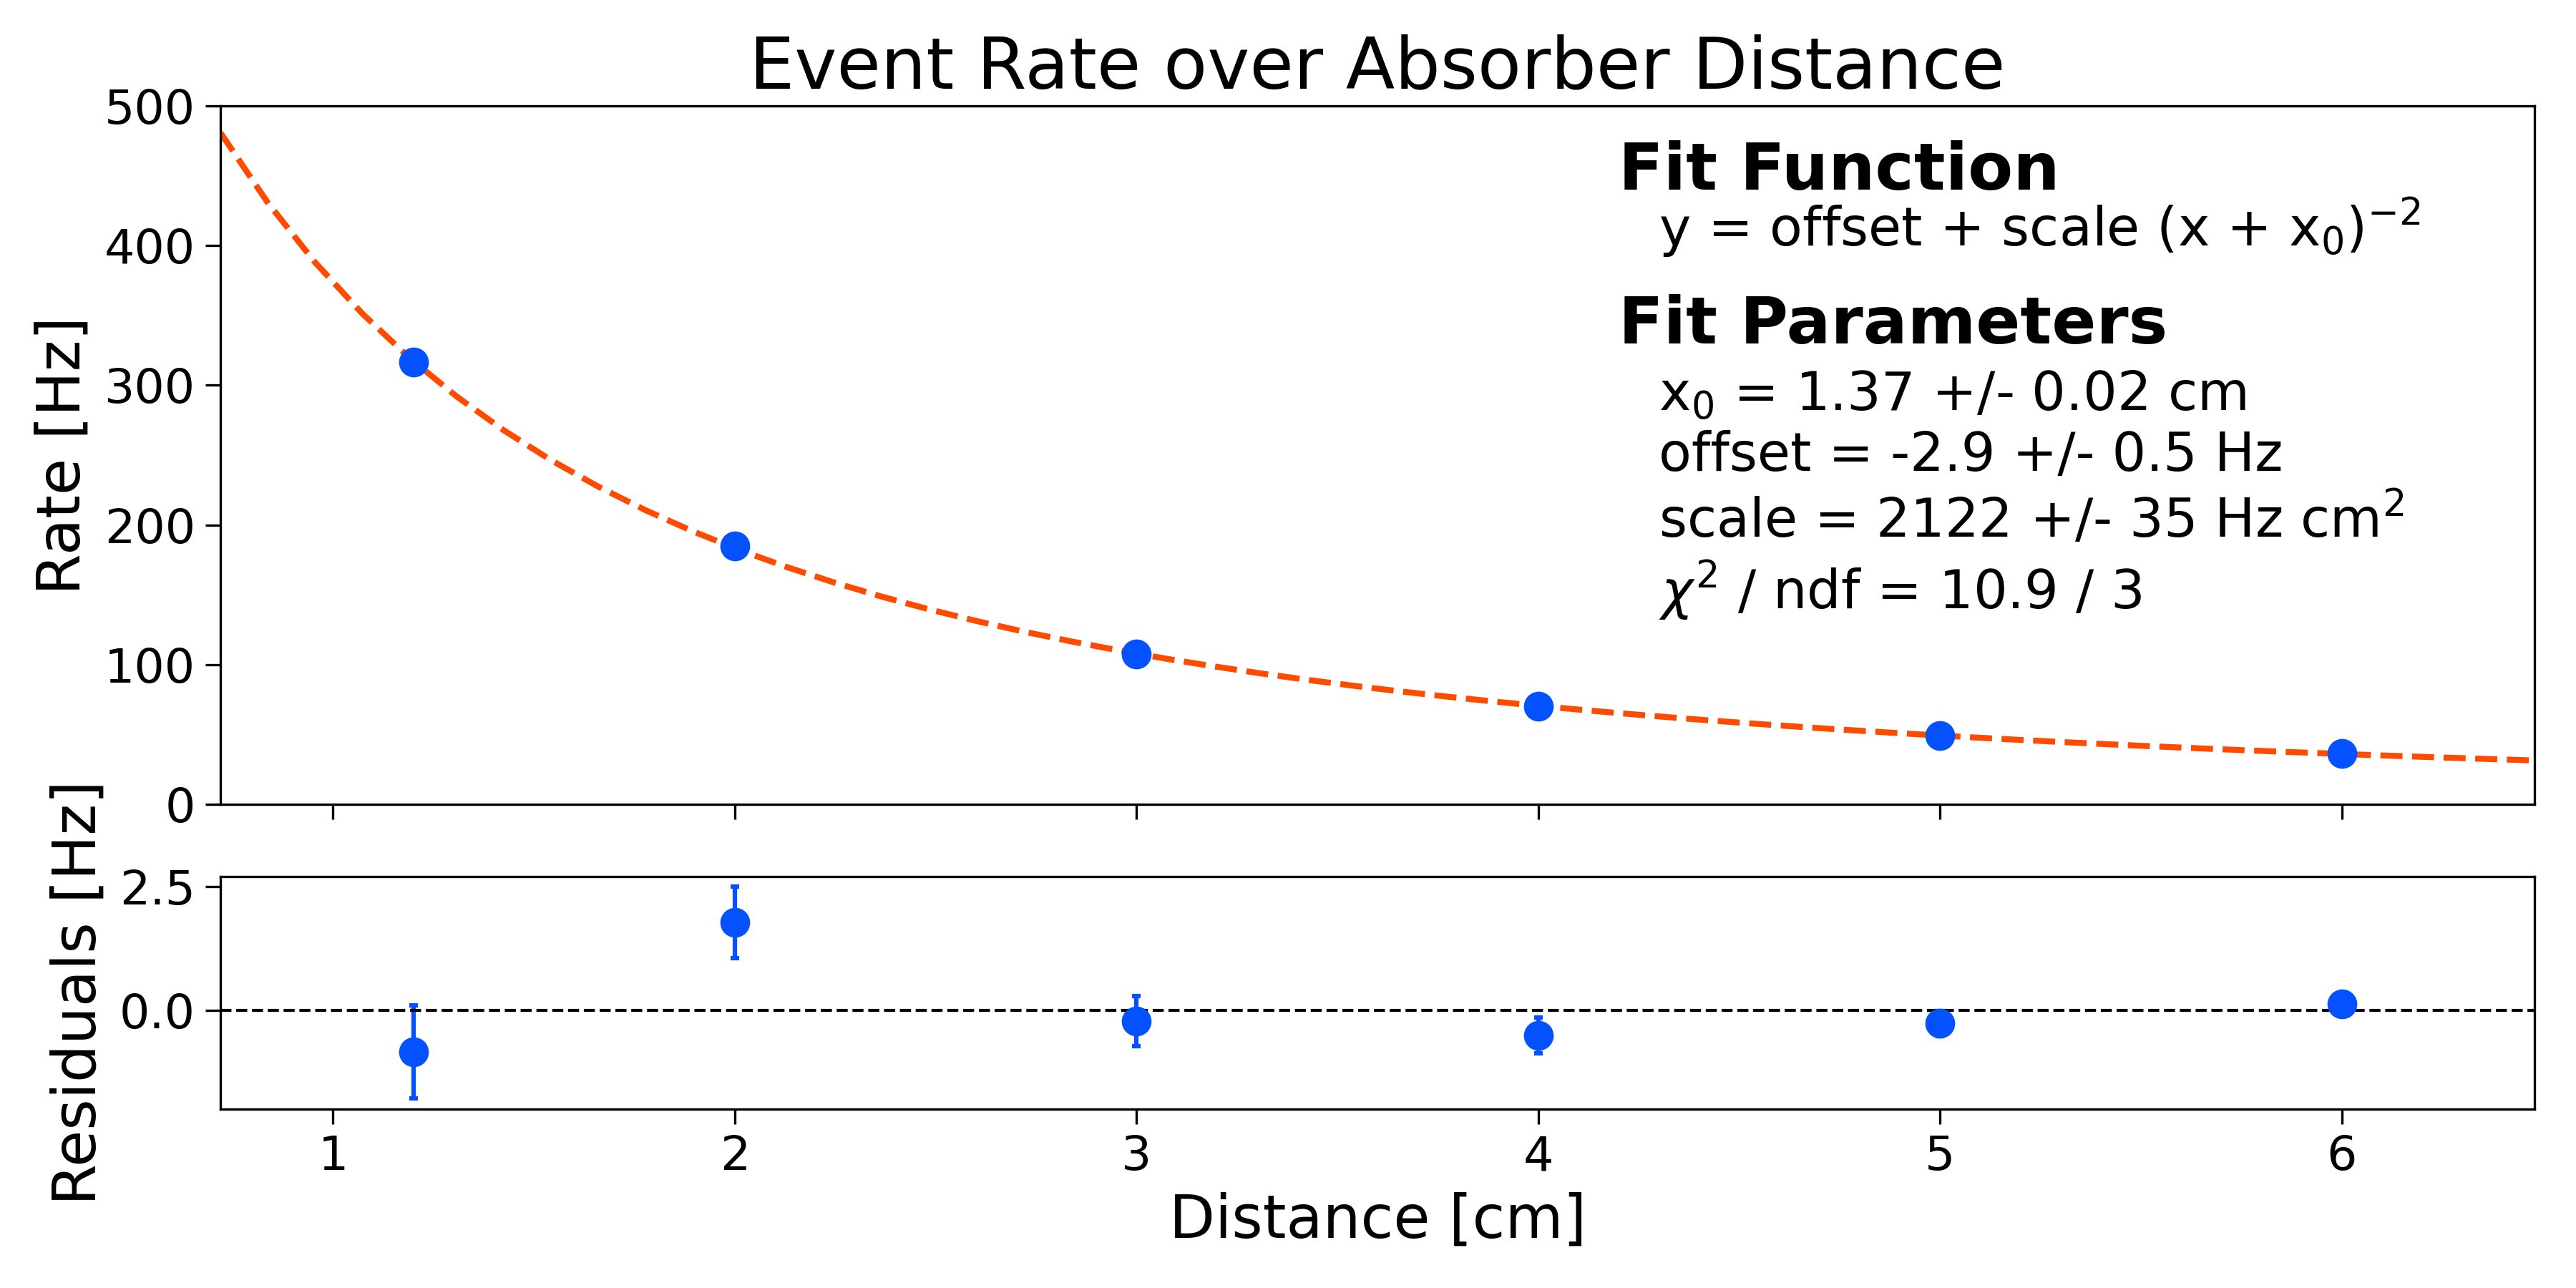
\includegraphics[width=\linewidth]{../Plots/distance_small.png}
    \caption{Rate di rivelazione dei raggi X in funzione della distanza tra sorgente e detector}
    \label{i:distance}
    \vspace{-10pt}
\end{figure}

Si riportano in \autoref{t:assorbimento} le coppie di dati utilizzati per la regressione, con errore sulle ordinate
calcolato per propagazione, trascurando le incertezze sui tempi di acquisizione. Infatti, siccome i valori dei tempi
restituiti dall'interfaccia del software si discostano senibilmente da quelli impostati manualmente, si è assunto un
errore massimo di $\Delta t = 0.1\,\si{\second}$, ed è stato preliminarmente verificato che tale contributo avesse un
peso relativo trascurabile. Si vuole inizialmente effettuare un fit esponenziale del tipo $y =
\text{I}_0\,\text{e}^{-\mu x}$. Successivamente, sfruttando il parametro $\text{I}_0$ per normalizzare i dati, si vuole
considerare il logaritmo del rate normalizzato ed effettuare una regressione lineare con la retta di equazione $y = mx$.
In questo modo i dati si distribuiscono secondo $\log(\text{I}/\text{I}_0)=-\mu x$, con errore sul logaritmo ottenuto
per propagazione.

In \autoref{t:parametri_mu} sono quindi riportati i risultati ottenuti attraverso i due fit. Si vuole ora quantificare
la bontà dei fit: nel caso dell'argento si nota che il $\chi^2$ risulta significativamente maggiore rispetto ai gradi di
libertà, sia nel fit esponenziale che in quello lineare (compatibilità rispettivamente $Z=5$ e $Z=3.7$). Tale
discrepanza può essere dovuta principalmente ad una leggera sottostima delle incertezze sul rate e al basso numero di
dati. Tuttavia, i residui si distribuiscono sufficientemente bene attorno allo zero, perciò la stima dei parametri è da
considerarsi valida. Per il rame, invece, si trova un ottimo accordo tra $\chi^2$ e numero di gradi di libertà
(compatibilità rispettivamente $Z=0.3$ e $Z=0.6$): infatti i dati seguono chiaramente l'andamento atteso e gli errori
sulle ordinate coprono bene la dispersione. 

In \autoref{t:results} si riportano le densità dei due materiali e le grandezze stimate a partire dai fit, assieme alla
compatibilità tra le stime sperimentali dei coefficienti di assorbimento massivi ed i valori teorici, assunti privi di
errore. 



\vspace{-10pt}
% %%%%%%%%%%%%%%%%%%%%%%%%%%%%%%%%%%%%%%%%%%%%%%%%%%%%%%%%%%%%%%%%%%%%%%
\section{Legge dell'Inverso del Quadrato della Distanza}\label{s:distanza}



\begin{table}[t]
	\centering
	\begin{tabular}{C{3cm} C{3cm}} 

        \toprule[0.5px]
        \toprule[0.1px]

		\multicolumn{2}{c}{\bfseries Rate in funzione della posizione} \tn

		\midrule[0.1px]

		Posizione [cm] & Rate [Hz] \tn

		\addlinespace

        $1.2$	&   $316.4	\pm 0.9$ \tn
        $2.0$	&   $185.2	\pm 0.7$ \tn
        $3.0$	&   $107.8	\pm 0.5$ \tn
        $4.0$	&   $70.1	\pm 0.4$ \tn
        $5.0$	&   $49.1	\pm 0.3$ \tn
        $6.0$	&   $36.2	\pm 0.2$ \tn

		\bottomrule[0.5px]		
	\end{tabular}
	\caption{Posizione del detector con associato il relativo rate di rivelazione}
	\label{t:distance}
    \vspace{-10pt}
\end{table}	

Ci si propone ora di verificare la cosiddetta "legge dell'inverso del quadrato della distanza". In particolare, si vuole
controllare che il rate dei raggi X (ovvero il primo picco a sinistra in \autoref{i:spettro}) segua un andamento
proporzionale all'inverso della distanza al quadrato tra sorgente e detector. In assenza di assorbitori tra i due,
quindi, vengono acquisiti una serie di spettri facendo variare la posizione del rivelatore. Dagli spettri acquisiti
viene calcolato il rate degli X: tali valori, assieme alla posizione del detector, sono riportati in
\autoref{t:distance}. Questi vengono quindi raffigurati in \autoref{i:distance}: si vuole far notare in particolar modo
la presenza di un parametro $x_0$ di zero. Infatti, tramite il software per la movimentazione del detector è possibile
unicamente impostarne la posizione lungo una rotaia: l'effettiva distanza con la sorgente è invece ignota a priori in
quanto la posizione della sorgente non corrisponde allo zero del sistema di riferimento utilizzato dal software per
posizionare il detector sulla guida. \\
Per la verifica della legge dell'inverso del quadrato della distanza si vuole quantificare la bontà del fit: il $\chi^2$
risulta sensibilmente maggiore rispetto ai gradi di libertà (compatibilità $Z=3$). Tuttavia, siccome nel caso in
questione non sono stati considerati numerosi effetti ulteriori e, possibilmente anche a causa dello scarso potere
risolvente dell'apparato, l'incertezza sul rate di rivelazione può essere stata (leggermente) sottostimata. In questo
caso, dunque, una compatibilità $Z=3$ con i gradi di libertà non è da considerarsi pessima: osservando il grafico dei
residui, infatti, si osserva un soddisfacente andamento attorno allo zero. Si può quindi concludere che le misure
acquisite al variare della distanza tra sorgente e detector seguono piuttosto fedelmente un andamento proporzionale
all'inverso della distanza al quadrato. 




\vspace{-10pt}
% %%%%%%%%%%%%%%%%%%%%%%%%%%%%%%%%%%%%%%%%%%%%%%%%%%%%%%%%%%%%%%%%%%%%%%
\section{Efficienza del Rivelatore}\label{s:efficienza}

\begin{figure*}[t]
    \centering
    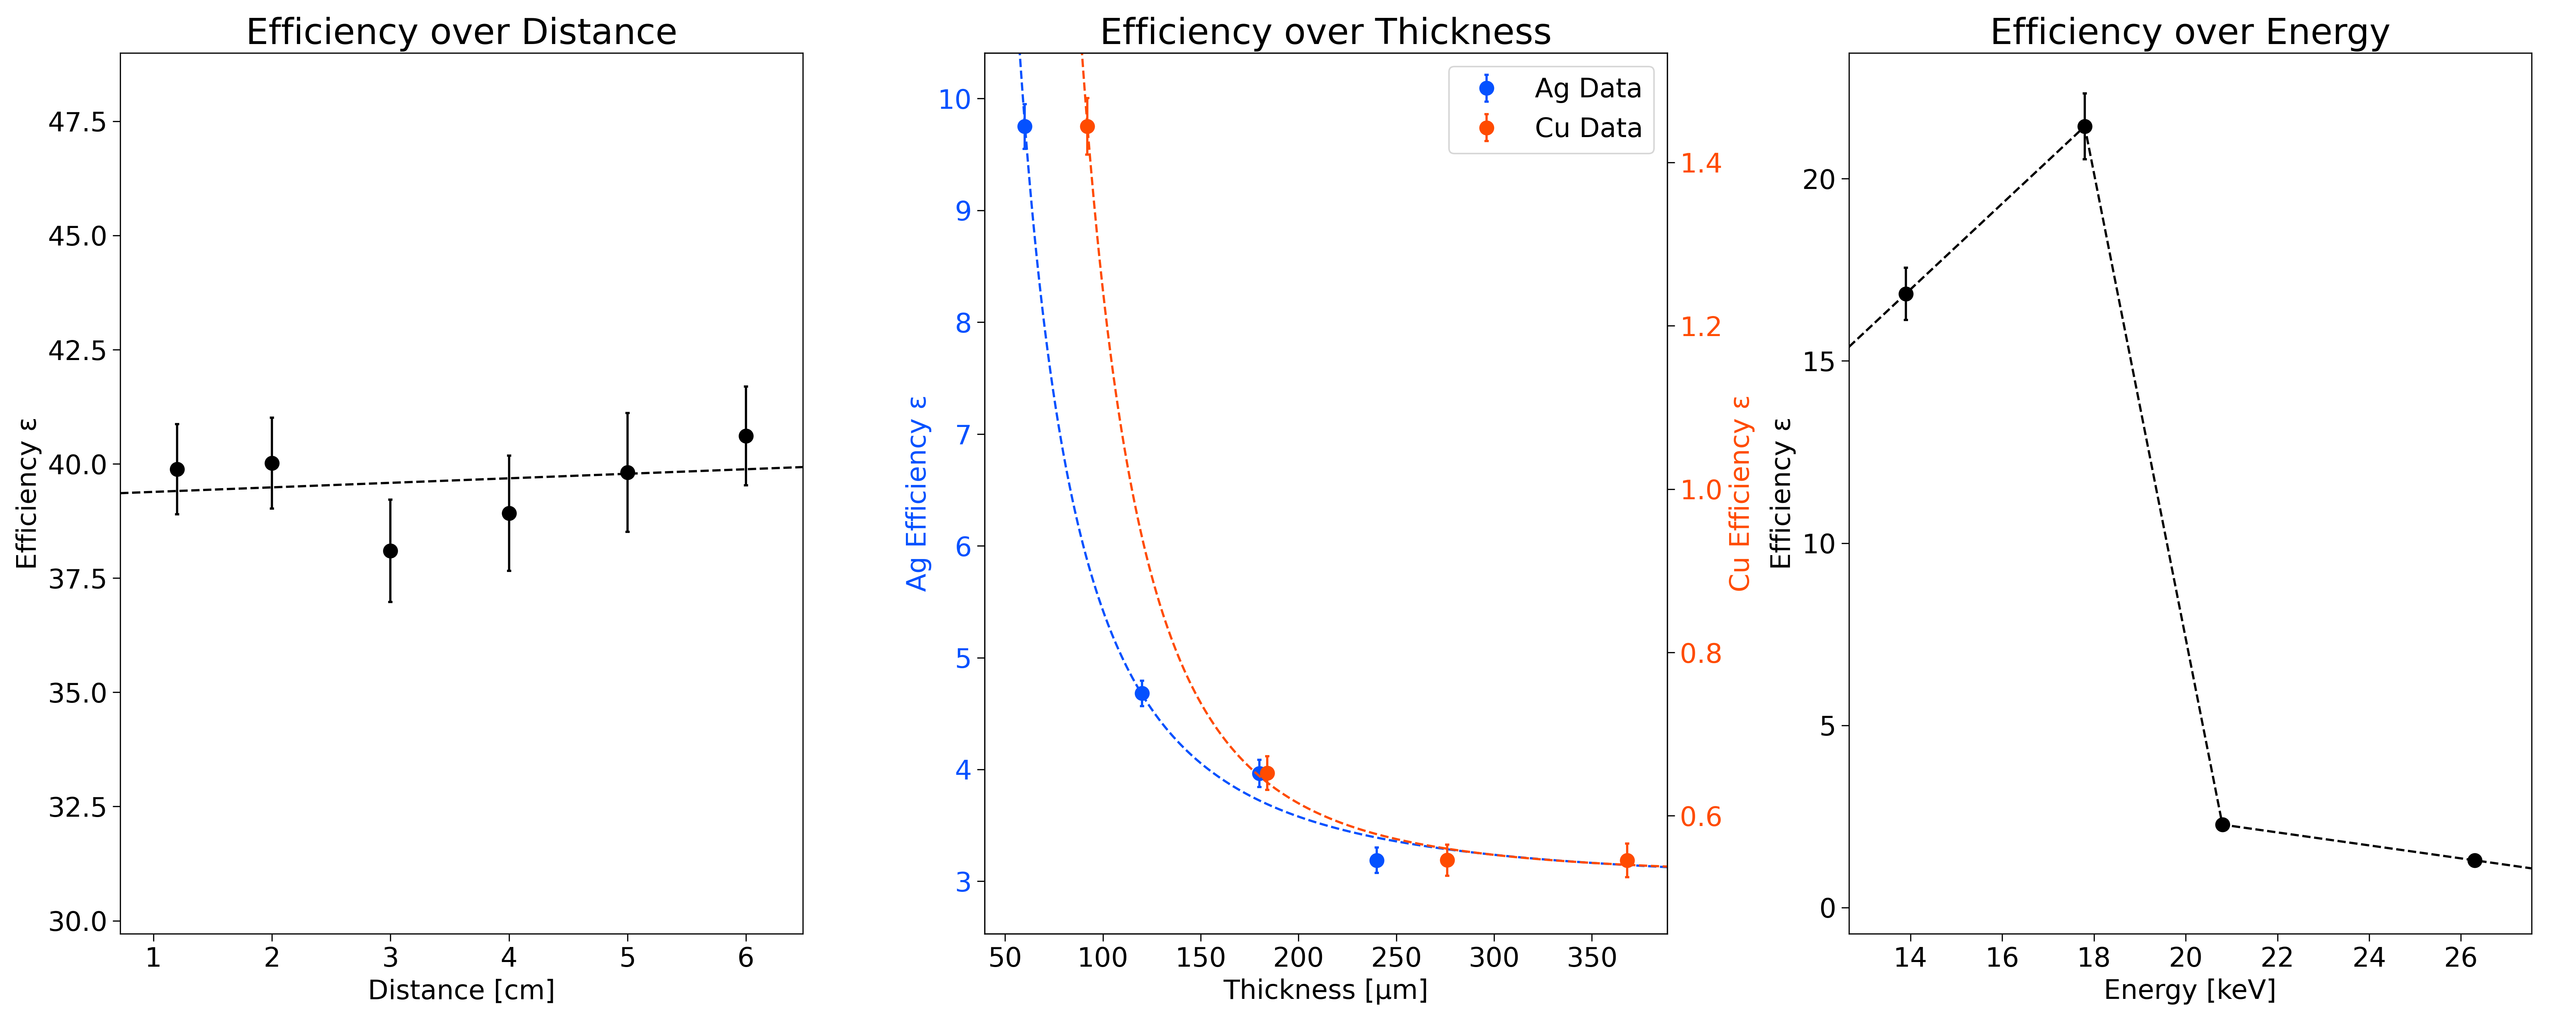
\includegraphics[width=\textwidth]{../Plots/efficiency.png}
   \caption{Curve di efficienza in funzione della distanza tra sorgente e detector (a sinistra), dello spessore di un
            assorbitore (in centro) e in funzione dell'energia dei fotoni (a destra)}
    \label{i:efficiency}
    % \vspace{-10pt}
\end{figure*}

In questa sezione finale ci si propone dapprima di calcolare l'efficienza del rivelatore legata al range di energie
degli X (il picco è costituito in realtà da più contributi distinti ma viene qui considerato come unico) relativamente
al picco situato a $60\,\si{\kilo\electronvolt}$. Non conoscendo l'attività della sorgente, infatti, non si è in grado
di stimare l'efficienza in modo indipendente da un picco di riferimento, e si è quindi costretti al calcolo di
un'efficienza relativa che si riduce ad un rapporto tra le aree dei due picchi. Siccome il metodo più preciso per il
calcolo dell'area è quello di sommare direttamente i bin nel range di energie del picco, non viene effettuato qui alcun
tipo di fit. Sfruttando allora l'acquisizione riportata in \autoref{s:spettro} si stima l'efficienza relativa

\vspace{-15pt}
\begin{equation}\label{e:efficienza}
    \epsilon_{\text{rel}} = \frac{\text{N}_{\text{X}}}{\text{N}_{\gamma}} = 42.0 \pm 0.6
    \vspace{-5pt}
\end{equation}

\subsection{Curve di Efficienza}

Si vogliono ora costruire delle curve di efficienza, con l'obiettivo di studiare l'andamento di quest'ultima al variare
di diverse quantità. In particolare, le curve che vengono qui trattate sono tre: la prima è relativa alla distanza tra
sorgente e detector, la seconda è relativa allo spessore di un assorbitore interposto tra sorgente e detector, mentre la
terza e più delicata è relativa all'energia del fotone rivelato. 

Per costruire la curva di efficienza al variare della distanza tra sorgente e rivelatore, vengono sfruttate le
acquisizioni riportate in \autoref{s:distanza}. In particolare, per ogni spettro raccolto viene calcolata l'efficienza
del picco degli X relativa al picco a $60\,\si{\kilo\electronvolt}$ come in \autoref{e:efficienza}. Per costruire poi la
curva di efficienza al variare dello spessore dell'assorbitore tra sorgente e rivelatore si utilizzano le acquisizioni
riportate in \autoref{s:attenuazione}. Si procede quindi in modo analogo alla costruzione della curva al variare della
distanza. Infine, si vuole ricavare la curva di efficienza in funzione dell'energia dei fotoni rivelati sfruttando  i
risultati ottenuti mediante il fit multi-picco in \autoref{i:multifit}. A causa dello scarso potere risolvente del
rivelatore, tuttavia, non è possibile isolare dall'istogramma i singoli contributi che compongono il picco degli X, e ci
si trova quindi costretti ad utilizzare le informazioni restituite dal fit. In questo caso, si continua a scegliere il
picco a $60\,\si{\kilo\electronvolt}$ come riferimento in quanto risulta essere l'unico picco ben risolto, dal quale
possiamo trarre informazioni più precise rispetto ai contributi non risolti. Per costruire la curva di efficienza,
quindi, viene calcolato il rapporto in \autoref{e:efficienza} per ciascun contributo di raggi X che compone il picco,
sfruttando però i parametri $\{N_i\}$, riportati in \autoref{i:multifit}, normalizzati con le rispettive probabilità di
emissione (\autoref{t:probabilities}). 

Le tre curve di efficienza sono riportate in \autoref{i:efficiency}: a sinistra si può osservare l'efficienza relativa
al variare della posizione del detector, in centro si trovano le due curve in funzione dello spessore dell'assorbitore
mentre a destra è raffigurata l'efficienza relativa in funzione dell'energia dei fotoni emessi. Osservando inizialmente
il primo grafico a sinistra, si può notare come l'efficienza segua un andamento piuttosto costante. Il valore medio è in
accordo con il risultato in \autoref{e:efficienza} (la lieve discrepanza può essere legata ad una statistica meno
elevata nell'acquisizione degli spettri al variare della distanza) e, inoltre, la fluttuazione statistica è
confrontabile con le incertezze dell'efficienza. Dalla costanza del rapporto di efficienza relativa
$\text{N}_{\text{X}}/\text{N}_{\gamma}$, si può quindi dedurre che la distanza tra sorgente e detector influenza in
ugual modo la rivelazione degli X e dei $\gamma$. Osservando invece il grafico centrale, è evidente come l'efficienza
relativa segua un forte andamento decrescente: in particolare, la differenza di andamento tra i due materiali è
influenzata dal diverso coefficiente di assorbimento. Il grafico prova chiaramente, quindi, che i raggi $\gamma$ sono
molto più penetranti rispetto agli X: dallo spettro in \autoref{i:spettro_abs}, infatti, si nota che in presenza di un
assorbitore di rame spesso $368\,\si{\micro\metre}$ il rapporto di rivelazione tra raggi X e raggi $\gamma$ è molto
diverso rispetto a quanto ritrovato in \autoref{i:spettro} senza assorbitore. Il picco corrispondente agli X, infatti,
risulta ora essere addirittura più basso del picco a $60\,\si{\kilo\electronvolt}$, evidenziando come i fotoni meno
energetici vengano bloccati più facilmente rispetto a quelli più energetici. Osservando infine il grafico a destra in
\autoref{i:efficiency}, ovvero la curva di efficienza in funzione dell'energia, è complicato trarre conclusioni data la
scarsa quantità di informazione a disposizione: i contributi gaussiani presi in considerazione non sono in numero
sufficiente da far emergere un trend evidente. Inoltre, il range di energie in gioco è piuttosto ristretto, ed il basso
potere risolvente dell'apparato costringe la curva ad essere fortemente dipendente dai parametri del fit multi-picco
(\autoref{i:multifit}), che descrive però in modo solo approssimativo il profilo dello spettro. Infatti, il grafico
evidenzia la stessa anomalia esposta in \autoref{s:multipicco}: il picco a $16.8\,\si{\kilo\electronvolt}$ risulta
essere estremamente sovrastimato. Infine, è opportuno evidenziare che per poter ricavare delle informazioni
soddisfacenti sull'efficienza del detector in funzione dell'energia, sarebbe necessario conoscere almeno l'attività
della sorgente. In questo modo, infatti, il numero di fotoni emessi dalla sorgente sarebbe una quantità calcolabile e,
conseguentemente, anche l'efficienza assoluta. 


\pagebreak

\begin{figure}[t]
    \centering
    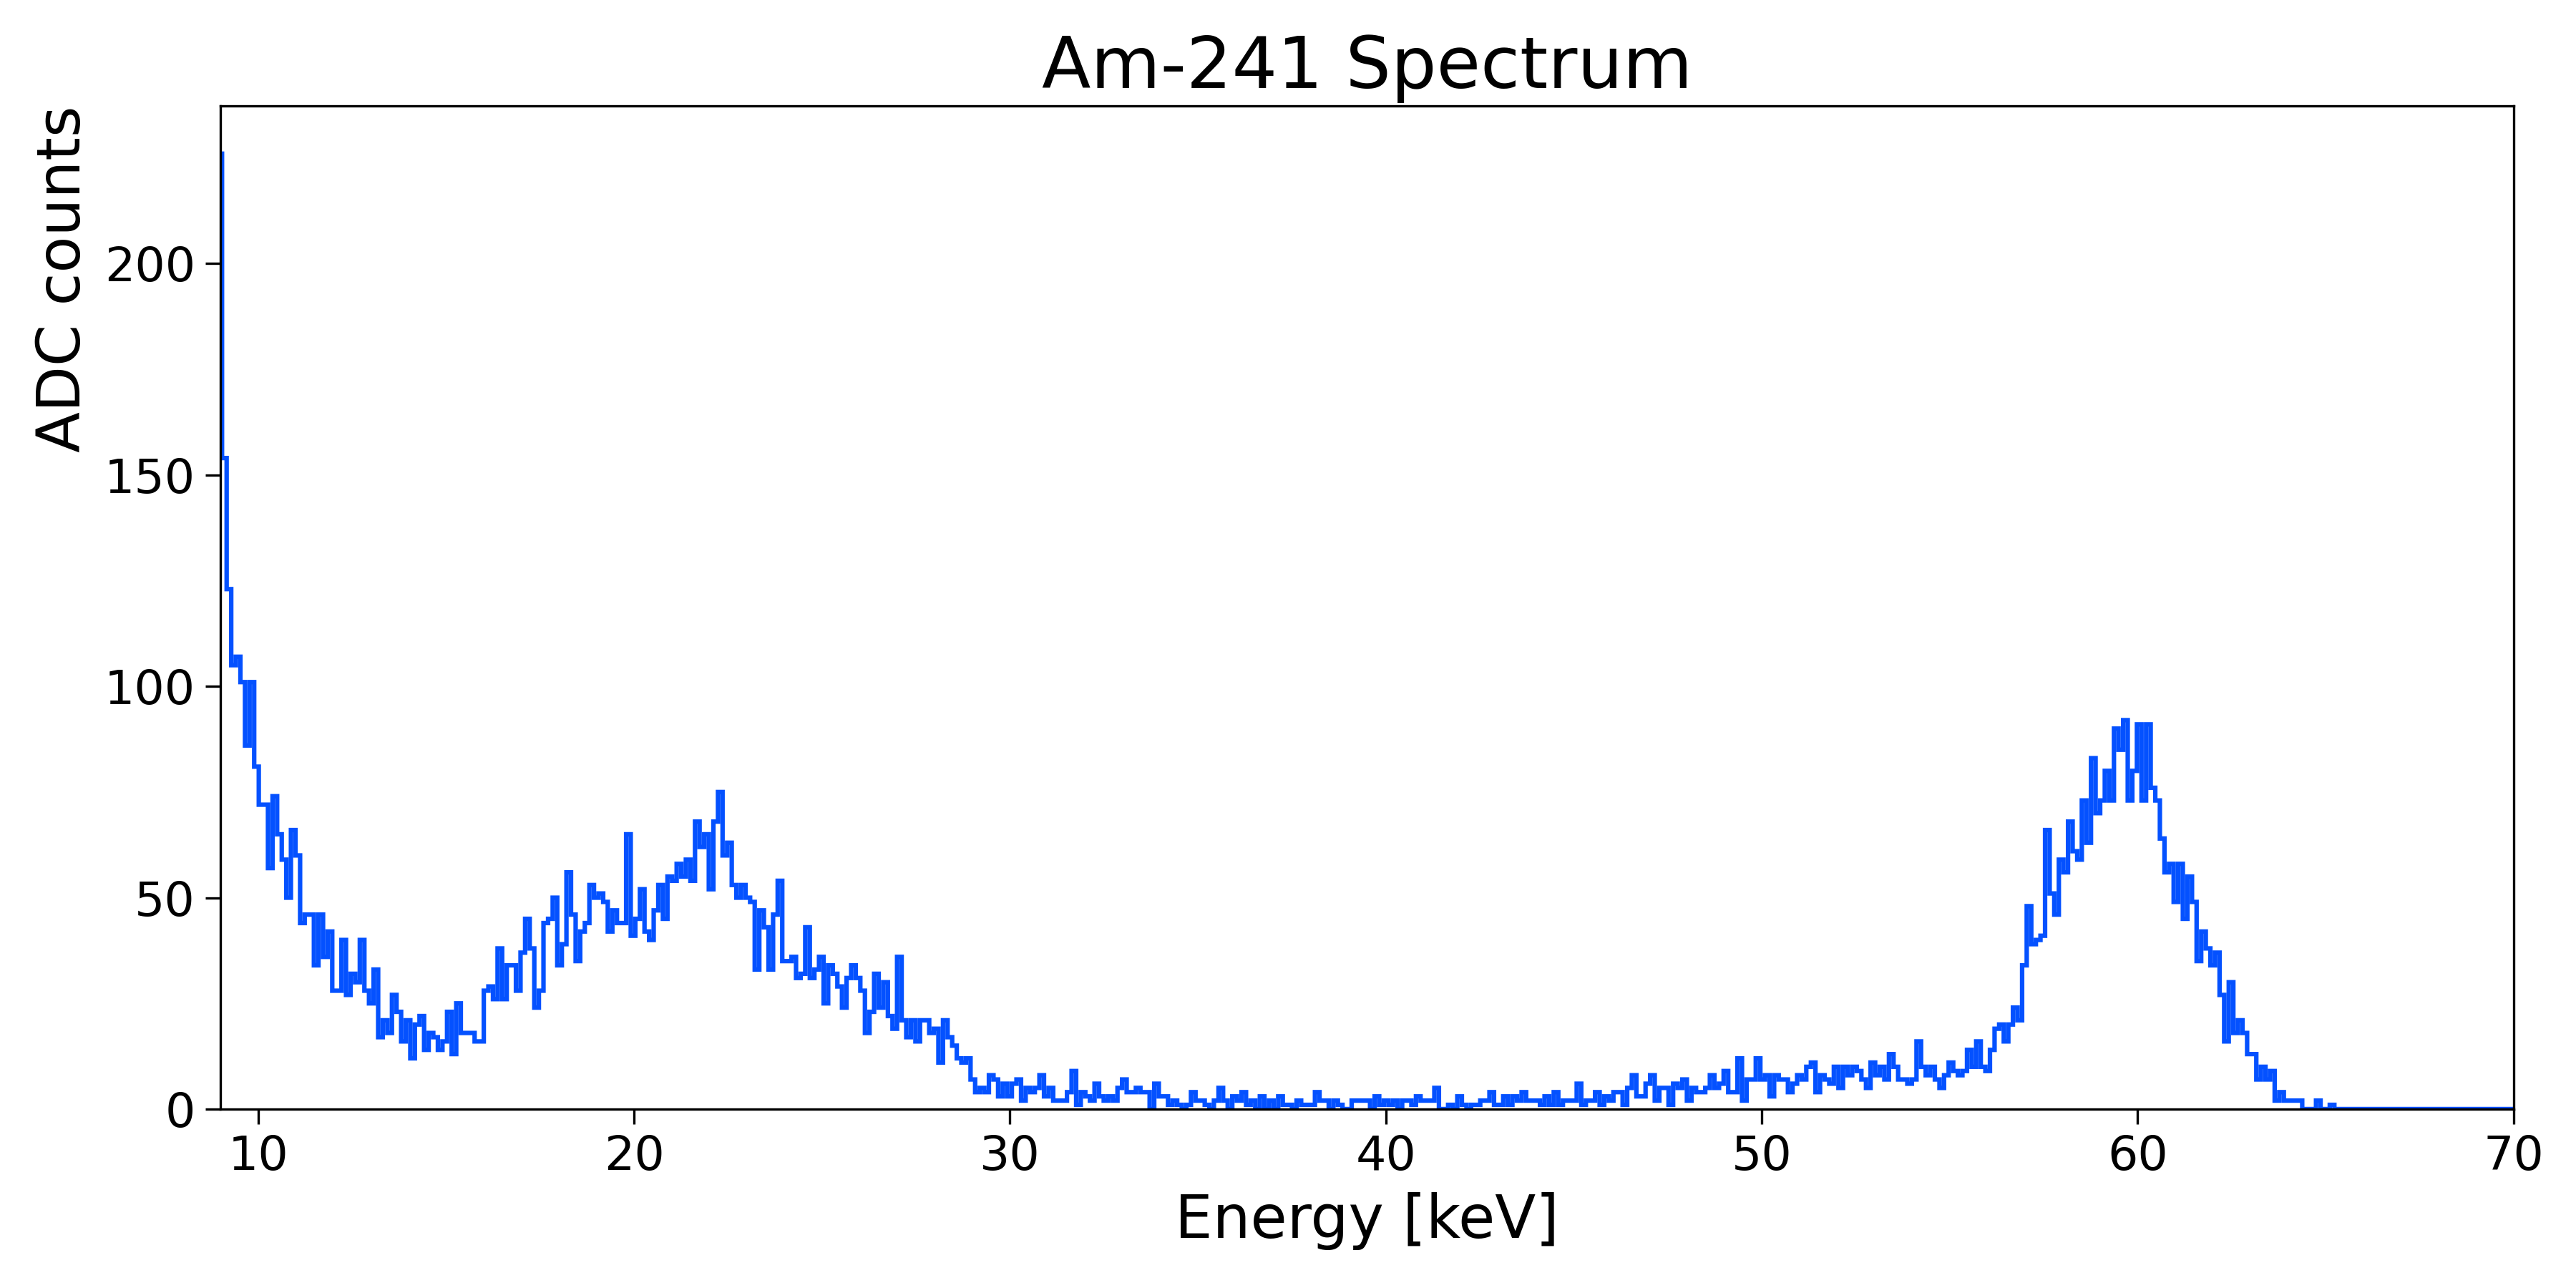
\includegraphics[width=\linewidth]{../Plots/am_spectrum_absorber.png}
    \caption{Spettro dell'Am-241 con assorbitore di rame di spessore $368\,\si{\micro\metre}$}
    \label{i:spettro_abs}
    \vspace{-15pt}
\end{figure}



\null
\vfill

\end{document}


					
